\documentclass[12pt,a4paper]{article}

% Packages
\usepackage{amsmath}
\usepackage{amsfonts}
\usepackage{amssymb}
\usepackage{graphicx}
\usepackage[margin=1in]{geometry}
\usepackage{enumitem}
\usepackage[hidelinks]{hyperref}
\usepackage{xcolor}

% Title
\title{Homework Report for Computer Vision}
\author{Yu Xiang, Luo}
\date{\today}

\begin{document}

\maketitle

\[
	\href{https://github.com/YuXiangLo/Computer-Vision}{\text{\textcolor{blue}{You can check this github for more information}}}
\]

\begin{itemize}
	\item Original Lena\\ 
		\\
		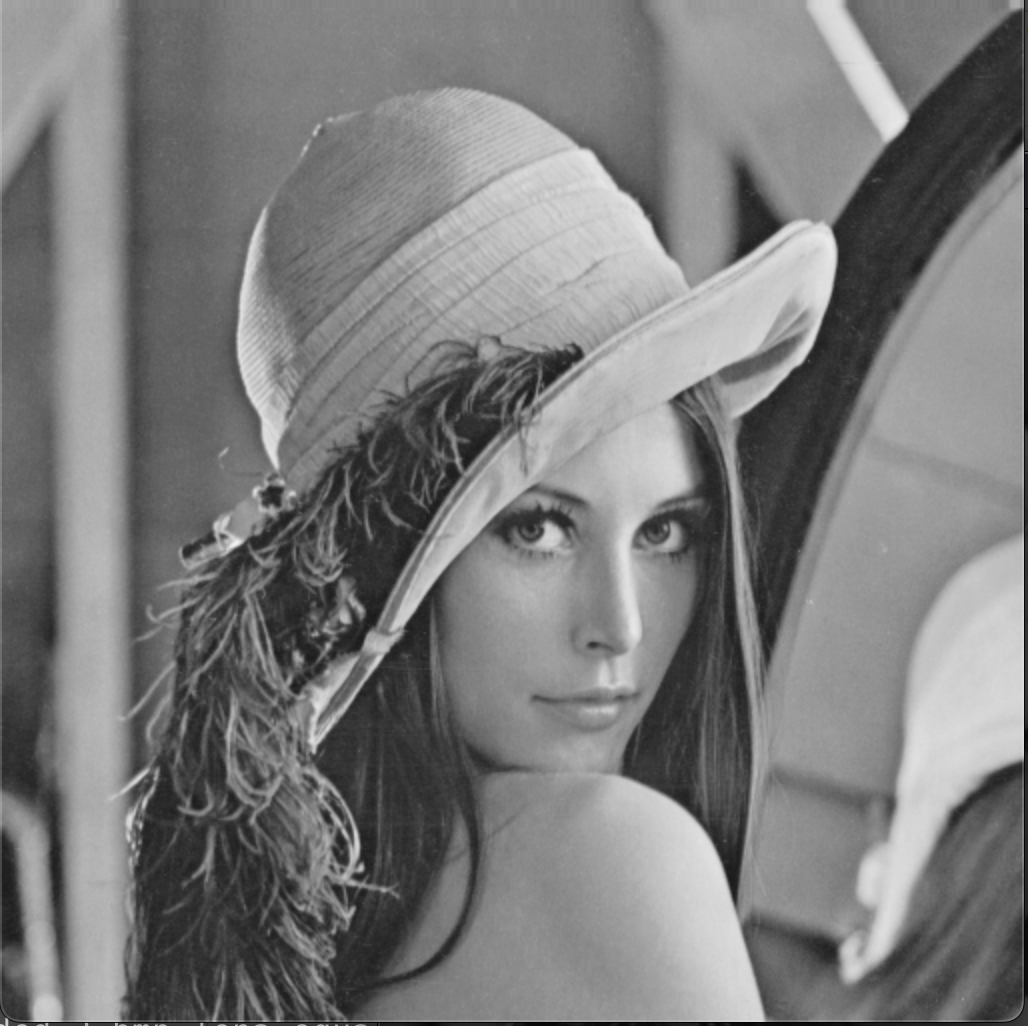
\includegraphics[width=0.45\textwidth]{./img/original_lena.png}
		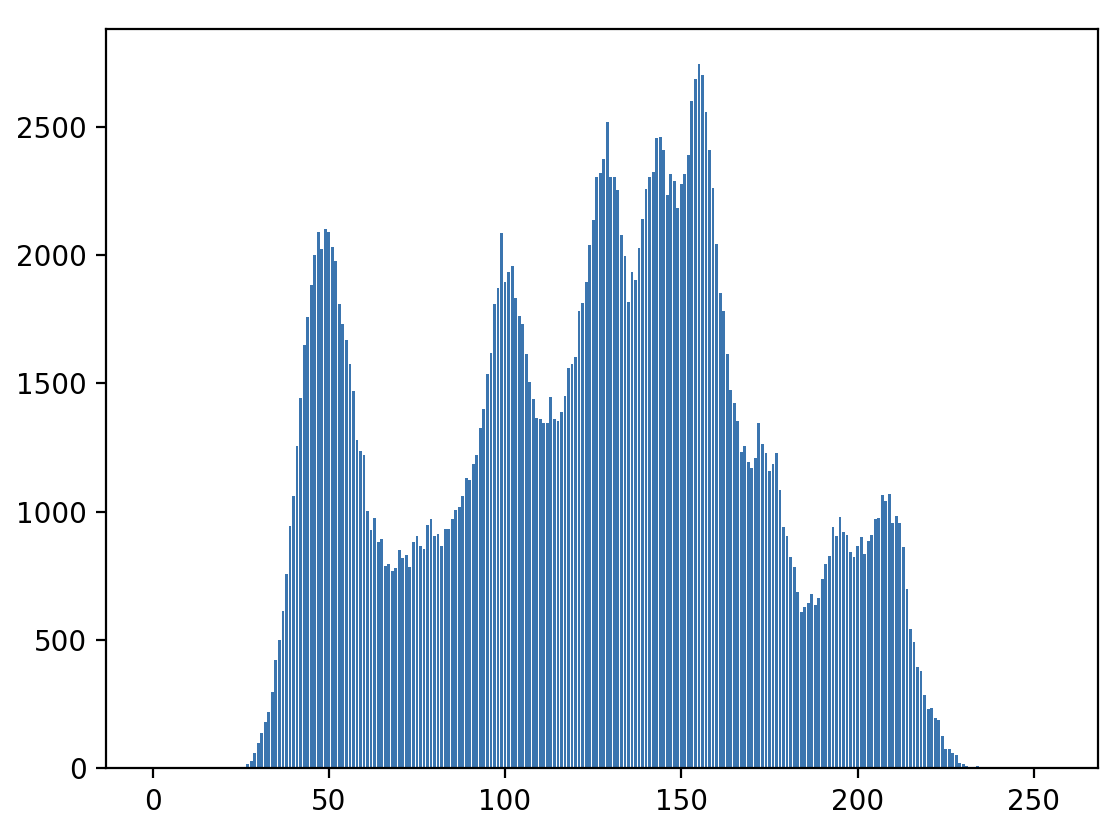
\includegraphics[width=0.5\textwidth]{./img/original.png}
	\item Intensity Divided by 3 Lena\\
		\\
		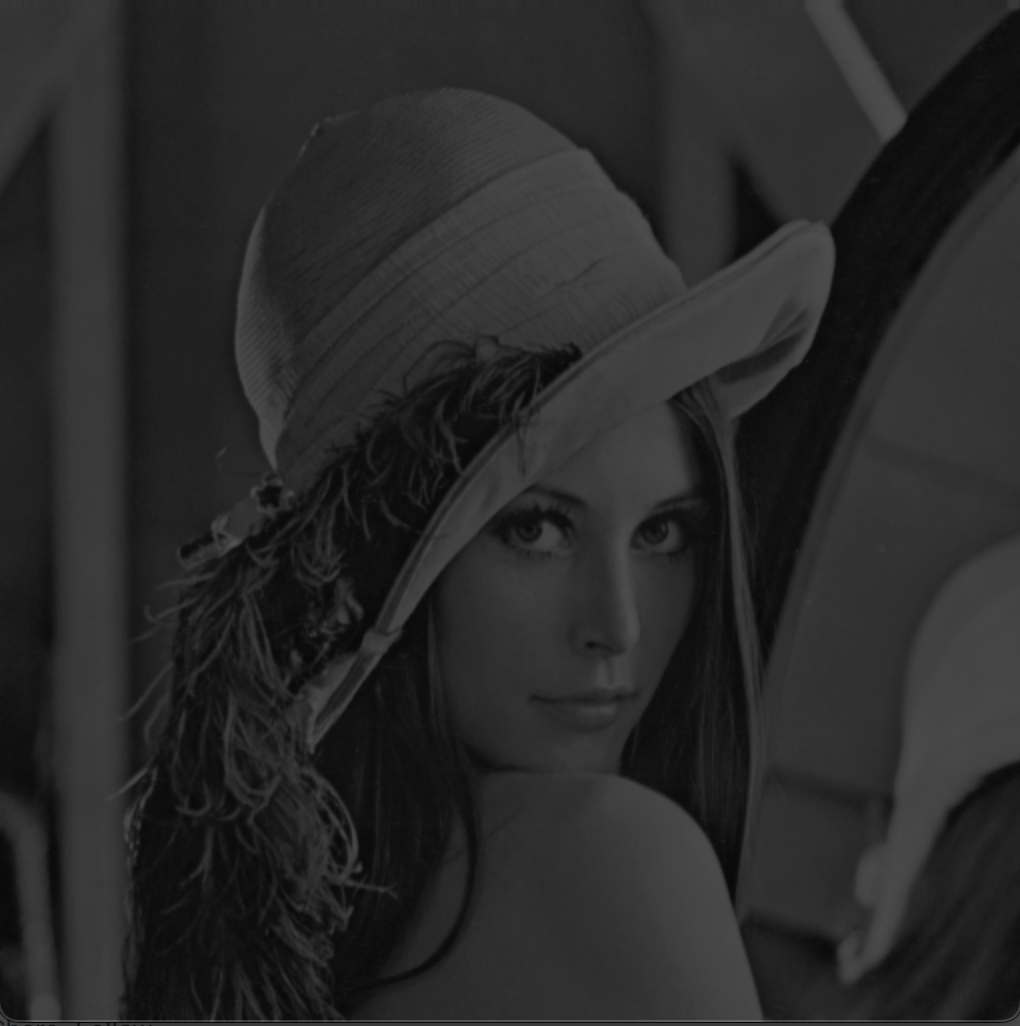
\includegraphics[width=0.45\textwidth]{./img/divide_3_lena.png}
		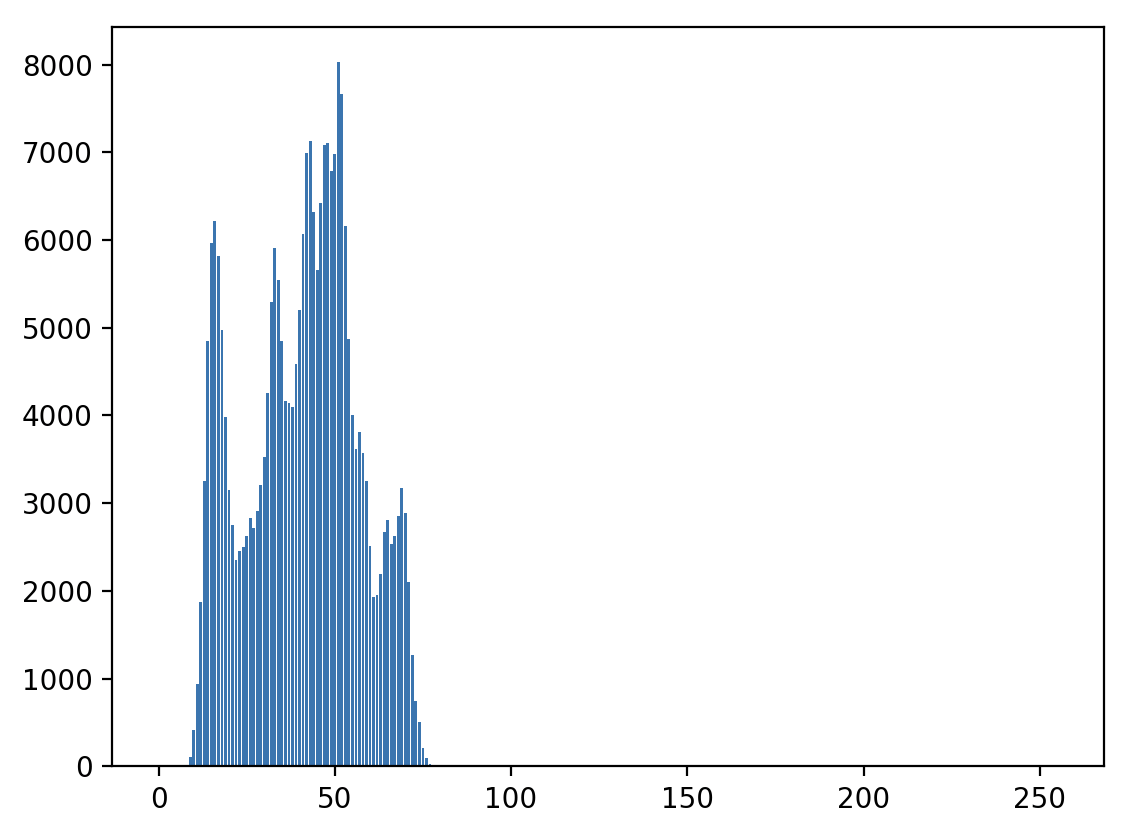
\includegraphics[width=0.5\textwidth]{./img/divide_3.png}
	\item Rescale \textcolor{gray}{(Histogram Equalization)} Lena\\
		\\
		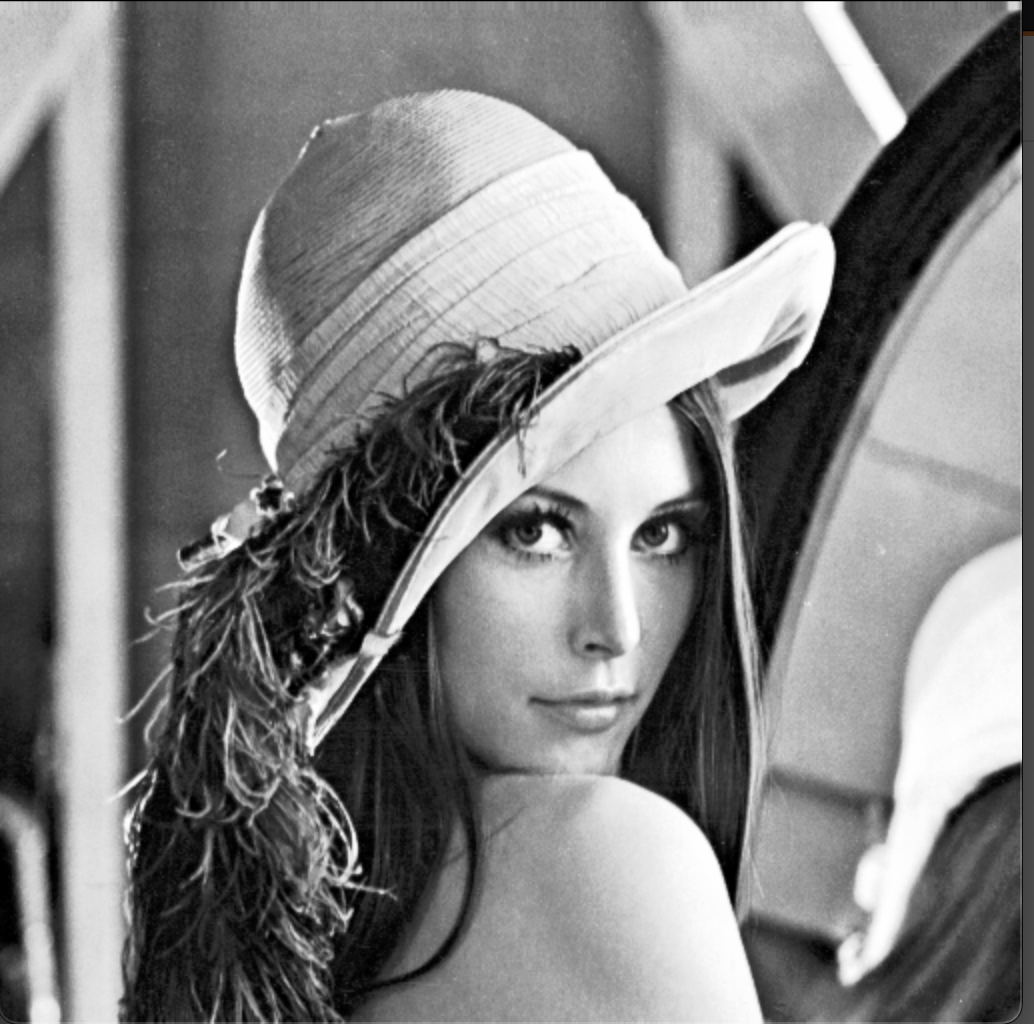
\includegraphics[width=0.45\textwidth]{./img/equal_lena.png}
		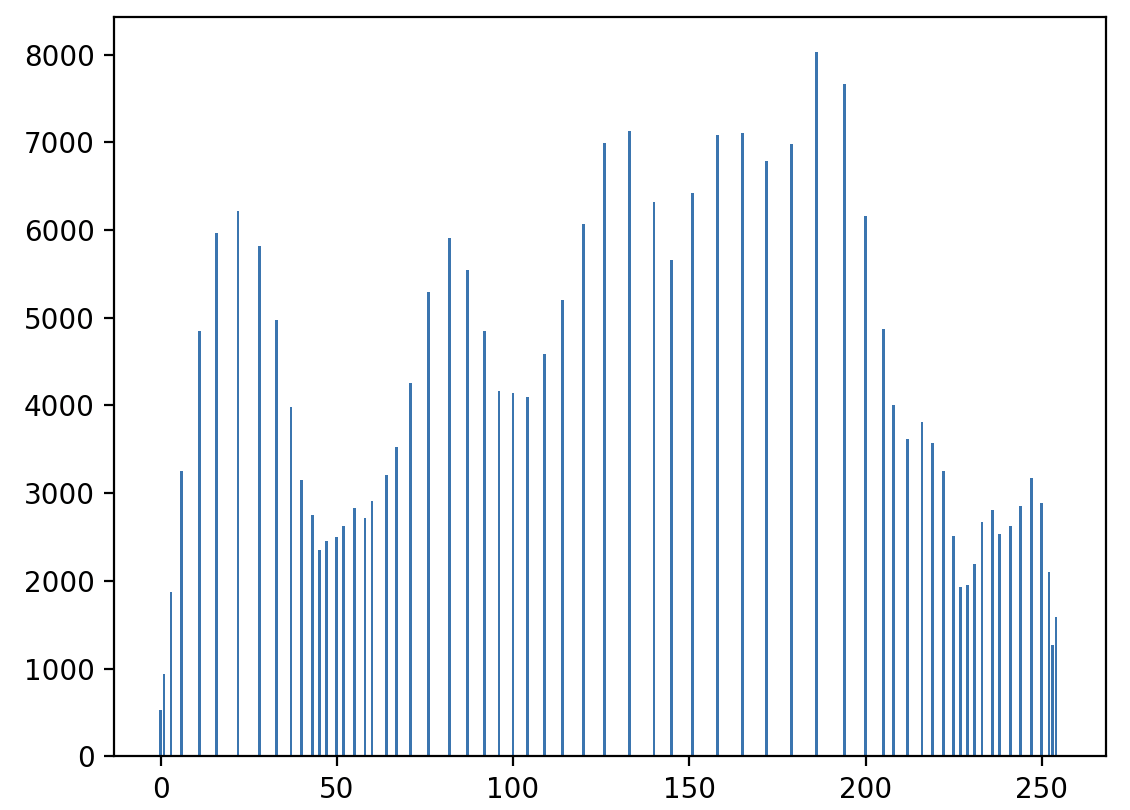
\includegraphics[width=0.5\textwidth]{./img/equalization.png}
		\[\fbox{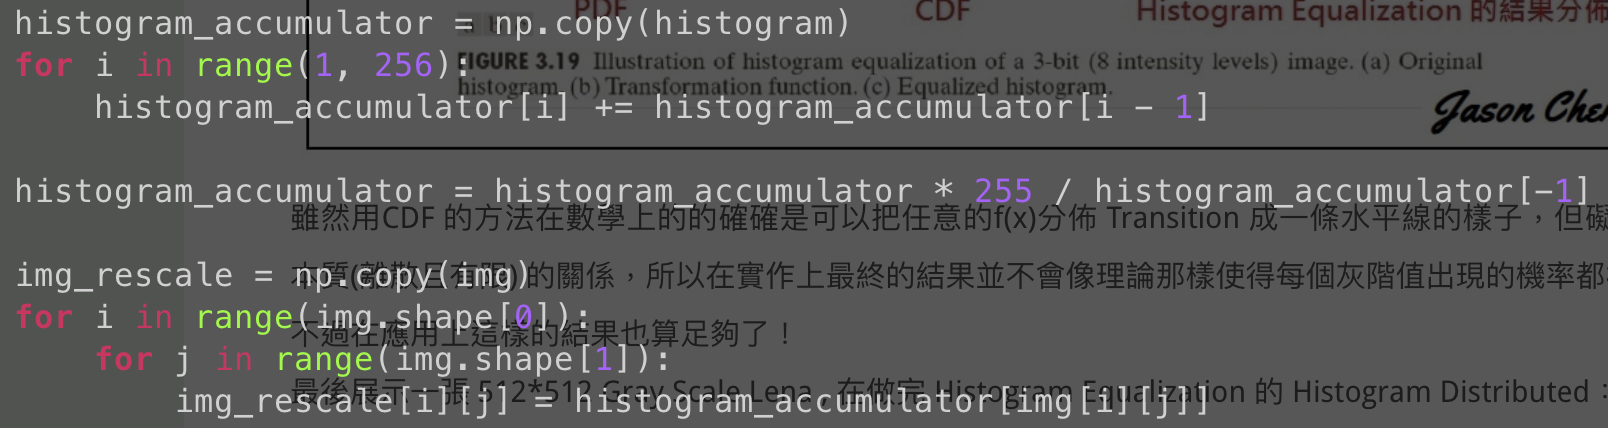
\includegraphics[width=0.8\textwidth]{./img/code.png}}\]
	Additional coding details can be located within the \textbf{HW3.py} file. This snippet is responsible for calculating the cumulative distribution function (CDF) and reorganizing it in such a way that the resulting CDF approaches a linear progression.
\end{itemize}



\end{document}
